\documentclass[a4paper, landscape]{article}

\usepackage{graphicx} % Allows including images
\usepackage{stackengine}
\usepackage{scalerel}
\usepackage{xcolor}
\usepackage{geometry}
\usepackage{multicol}
\usepackage{listings}

\graphicspath{{./../img/}}
\renewcommand{\abstractname}{}
\renewcommand{\tt}[1]{\texttt{#1}}

\newcommand\dangersign[1][2ex]{%
  \renewcommand\stacktype{L}%
  \scaleto{\stackon[1.3pt]{\color{red}$\triangle$}{\tiny !}}{#1}%
}

\newcommand{\warn}[1]{\begin{center}
\begin{tabular}{ c  p{12cm} }
\dangersign[22pt] & \vspace{-0.6cm} #1
\end{tabular}
\end{center}}

\geometry{
 a4paper,
 left=30mm,
 right=30mm,
 top=30mm,
 bottom=30mm
 }

\lstset{language=Python,
		commentstyle=\color{gray},
		keywordstyle=\color{blue},
		numberstyle=\color{yellow},
		stringstyle=\color{purple}
}

\geometry{left=1cm,
			right=1cm,
			top=1cm,
			bottom=1cm}

\title{theia Quick Reference}

\begin{document}

\begin{tabular}{| p{.6cm} | p{7cm}| p{6cm} | p{5cm} |}
\hline
\textbf{Key} & \textbf{Input Order} & \textbf{Defaults} & \textbf{Remarks} \\ \hline \hline

\tt{bm} & \tt{Wx}, \tt{Wy} (waist sizes), \tt{WDistx}, \tt{WDisty} (waist positions from beam origin), \tt{Wl}, \tt{P}, \tt{X}, \tt{Y}, \tt{Z} (position of origin in space), \tt{Theta}, \tt{Phi} (orientation), \tt{Alpha} (rotation of eigenbase for orthogonal beams), \tt{Name}, \tt{Ref}  & \tt{Wx}~=~1.mm, \tt{Wy}~=~1.mm, \tt{WDistx}~=~0., \tt{WDisty}~=~0., \tt{Wl}~=~1064.nm, \tt{P}~=~1.W, \tt{X}~=~0., \tt{Y}~=~0., \tt{Z}~=~0., \tt{Theta}~=~pi/2., \tt{Phi}~=~0., \tt{Alpha}~=~0., \tt{Name}~=~"Beam", \tt{Ref}~=~None & \tt{Alpha = 0.} $\leftrightarrow$ eigen X is $\perp$ to beam direction and has maximum $Z$ component. If direction is $\pm e_Z$ then eigen X is $\pm e_X$\\ \hline

\tt{mr} & \tt{X}, \tt{Y}, \tt{Z} (position of center of HR chord), \tt{Theta}, \tt{Phi} (orientation of HR Norm, pointing out), \tt{Wedge}, \tt{Alpha} (wedge and wedge rotation), \tt{HRK}, \tt{ARK} (curvatures), \tt{Diameter}, \tt{Thickness} (of the construction cylinder), \tt{N}, \tt{HRr}, \tt{HRt}, \tt{ARr}, \tt{ARt} (power reflectances and transmittances), \tt{KeepI}, \tt{Name}, \tt{Ref} & \tt{X}~=~0., \tt{Y}~=~0., \tt{Z}~=~0., \tt{Theta}~=~pi/2., \tt{Phi}~=~0., \tt{Wedge}~=~0., \tt{Alpha}~=~0., \tt{HRK}~=~0.01, \tt{ARK}~=~0., \tt{Diameter}~=~10.cm, \tt{Thickness}~=~2.cm, \tt{N}~=~1.4585, \tt{HRr}~=~.99, \tt{HRt}~=~.01, \tt{ARr}~=~.1, \tt{ARt}~=~.9, \tt{KeepI}~=~False, \tt{Name}~=~"Mirror", \tt{Ref}~=~None & Wedges are counted positive if you \textit{add} material when you increase the wedge.\\ \hline

\tt{th} & \tt{X}, \tt{Y}, \tt{Z} (position of center of lens), \tt{Theta}, \tt{Phi} (orientation of HR Norm, pointing out), \tt{Focal} (focal length),  \tt{Diameter}, \tt{R}, \tt{T} (power reflectance and transmittance), \tt{KeepI}, \tt{Name}, \tt{Ref} & \tt{X}~=~0., \tt{Y}~=~0., \tt{Z}~=~0., \tt{Theta}~=~pi/2., \tt{Phi}~=~0., \tt{Focal}~=~10.cm,  \tt{Diameter}~=~5.cm, \tt{R}~=~.1, \tt{T}~=~.9, \tt{KeepI}~=~False, \tt{Name}~=~"Thinlens", \tt{Ref}~=~False & All parameters which are not present here are internally ajusted in order to fit the input \tt{Focal}, \tt{Diameter} and a \tt{N}~=~1.4584 value for the optical index\\ \hline

\tt{tk} & \tt{X}, \tt{Y}, \tt{Z} (position of apex of HR face of lens), \tt{Theta}, \tt{Phi} (orientation of HR Norm, pointing out), \tt{K1}, \tt{K2} (curvatures), \tt{Diameter},  \tt{Thickness}, \tt{N}, \tt{R}, \tt{T} (power reflectance and transmittance), \tt{KeepI}, \tt{Name}, \tt{Ref} & \tt{X}~=~0., \tt{Y}~=~0., \tt{Z}~=~0., \tt{Theta}~=~pi/2., \tt{Phi}~=~0., \tt{K1}~=~.01, \tt{K2}~=~.001, \tt{Diameter}~=~5.cm,  \tt{Thickness}~=~2.cm, \tt{N}~=~1.4585, \tt{R}~=~.1, \tt{T}~=~.9, \tt{KeepI}~=~False, \tt{Name}~=~"Thicklens", \tt{Ref}~=~None & \tt{Thickness}: on optical axis (from apex to apex) \\ \hline

\tt{bd} & \tt{X}, \tt{Y}, \tt{Z} (position of center of HR), \tt{Theta}, \tt{Phi} (orientation of HR Norm, pointing out), \tt{Diameter},  \tt{Thickness}, \tt{Name}, \tt{Ref} & \tt{X}~=~0., \tt{Y}~=~0., \tt{Z}~=~0., \tt{Theta}~=~pi/2., \tt{Phi}~=~0., \tt{Diameter}~=~5.cm,  \tt{Thickness}~=~2.cm, \tt{Name}~=~"BeamDump", \tt{Ref}~=~None & \\ \hline

\end{tabular}

\begin{multicols}{2}

\paragraph{Units.}(km, m = 1., cm, mm, um, nm), (kW, W = 1., mW, uW, nW), (THz, GHz, MHz, kHz, Hz = 1., mHz, uHz), (ppm = 1.e-6, rad = 1., deg), pi
\paragraph{Functions.} sin, cos, tan, arcsin, arccos, arctan, sqrt, exp

\paragraph{Notes.}\begin{itemize}
\item \tt{Theta}, \tt{Phi} are spherical coordinates around $e_Z$ and \tt{Phi = 0.} $\leftrightarrow~ + e_X$ 
\item All constructors can be called without arguments, all parameters have default values.
\end{itemize}

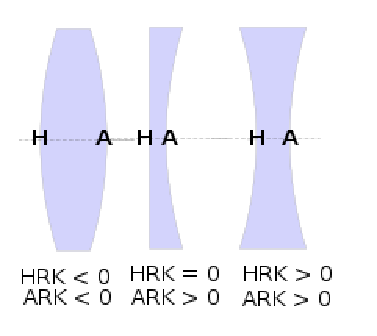
\includegraphics[scale=.6]{convention.pdf}
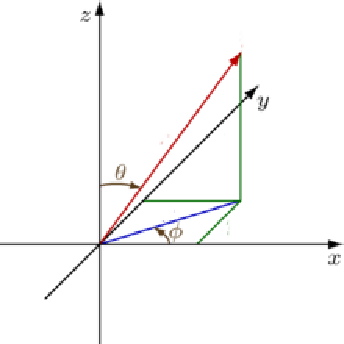
\includegraphics[scale=.6]{spherical.pdf}



\end{multicols}
\end{document}

